%%%%%%%%%%%%%%%%%%%%%%%%%%%%%%%%%%%%%%%%%%%%%%%%%%%%%%%%%%%%%%%%%%%%
%%%%%%%%%%%%%%%%%%%%%%%%%%%%%%%%%%%%%%%%%%%%%%%%%%%%%%%%%%%%%%%%%%%%
% BSS Seminar Paper Template 
% © Fynn Lohre 
%
% In case of any questions, reach out to: VARFynn@gmail.com.
%
%%%%%%%%%%%%%%%%%%%%%%%%%%%%%%%%%%%%%%%%%%%%%%%%%%%%%%%%%%%%%%%%%%%%
%%%%%%%%%%%%%%%%%%%%%%%%%%%%%%%%%%%%%%%%%%%%%%%%%%%%%%%%%%%%%%%%%%%%


%------------------------------------------------------------------%
% 1. Required Packages
% Add packages and, additonally, customize included ones.
%------------------------------------------------------------------%

\documentclass[12pt,a4paper]{article}
\usepackage[
	left 	= 2.5cm,
	right 	= 2.5cm, 
	top 		= 2.5cm,
	bottom 	= 2.5cm,
]{geometry}
\usepackage[utf8]{inputenc}
\usepackage[english]{babel}
\usepackage[OT1]{fontenc}
\usepackage{amsmath}
\usepackage{mathtools}
\usepackage{graphicx}
\usepackage{caption}
\usepackage[round]{natbib}
\usepackage{titlesec,xcolor}
\usepackage[hidelinks]{hyperref}
\hypersetup{
	colorlinks = true,
	urlcolor   = blue,
	linkcolor  = black, 
	citecolor  = blue, 
}
\newcommand{\mylink}[2]{\hyperref[#1]{\textcolor{blue}{#2}}}
% This allows you to link e.g. to figures: \mylink{F:2}{Figure 2}

\usepackage{fancyhdr}
\pagestyle{fancy}

% Formatting of the Sections has to be customized here
\usepackage{titlesec,xcolor}
\titleformat{\section}{\bfseries}{\thesection}{0.5em}{}
\titlespacing{\section}{0pt}{3ex plus 1ex minus 0.2ex}{10pt}
\setlength{\headheight}{14.49998pt}

\titleformat{\subsection}{\bfseries}{\thesubsection}{0.5em}{}
\titlespacing{\subsection}{0pt}{3ex plus 1ex minus 0.2ex}{10pt}
\setlength{\headheight}{14.49998pt}


%------------------------------------------------------------------%
% 2. Customizables
%------------------------------------------------------------------%
% Insert Name
\newcommand{\myname}{Fynn Lohre}

% Insert Title
\newcommand{\mytitle}{Bad Air Day: The Influence of Air Pollution on Quarterbacks' Performance - Evidence from the NFL}

% Insert Examiner
\newcommand{\myexaminer}{Professor Timo Hener, Ph.D. }

% Insert Course
\newcommand{\mycourse}{5440: Environmental Economics}

% Insert Submission Date
\newcommand{\mysubmission}{15.12.2023}

% Insert Matricle Nr. 
\newcommand{\mymatr}{202300181}

% Insert a "Display Name" of your paper (will be shown on the l.h.s. 
% of a certain page) - e.g. Doe 2014
\newcommand{\mypaper}{Lohre, 2023}



% If you want, you can customize the header
\author{\myname}
\title{\mytitle}
\lhead{\slshape \mypaper}
\chead{}
\rhead{\slshape \nouppercase{\leftmark}}


%------------------------------------------------------------------%
% 3. Content 
%------------------------------------------------------------------%
\begin{document}

%------------------------------------------------------------------%
% 3.1. Title Page
%------------------------------------------------------------------%
\begin{titlepage}
\center
\vfill

\includegraphics[scale=0.90]{BSS.png}
\vfill
\begin{tabular}[t]{lc}
Course:  & \mycourse \\
Examiner: & \myexaminer \\
Submission date: & \mysubmission \\
\end{tabular}
\vfill
{\large \textbf{\mytitle}}
\vfill
by \\ \vspace{3mm}
{\Large \myname}\\
(Student number \mymatr)\
\vfill
The relevant Data and Code are publicly available at \url{https://github.com/VARFynn/University_Contributions/tree/main/01_Master/02_Paper/Environmental_Econ_Paper}\\ 
\href{https://github.com/VARFynn/University_Contributions/tree/main/01_Master/02_Paper/Environmental_Econ_Paper}{
\includegraphics[scale=0.015]{GitHub.png}}
\vfill 
\thispagestyle{empty}
\pagebreak
\end{titlepage}

%------------------------------------------------------------------%
% 3.2. Abstract
%------------------------------------------------------------------%
\newcounter{savepage}
\pagenumbering{roman}
\thispagestyle{empty}
\begin{abstract}
\textit{Insert Your Abstract here. } 
\end{abstract}
\clearpage

%------------------------------------------------------------------%
% 3.3. TOC + Content
%------------------------------------------------------------------%
\thispagestyle{plain}
\tableofcontents
%\clearpage
%\listoftables
%\listoffigures
\pagebreak
\setcounter{savepage}{\arabic{page}}
\pagenumbering{arabic}
\section{Introduction}
\clearpage
\section{Theoretical Framework}
\clearpage
\section{Data and Descriptive Statistics}
\clearpage
\section{Empirical Framework}
\clearpage
\section{Results and Discussion}
\clearpage
\section{Summary and Concluding Remarks}
\clearpage


%------------------------------------------------------------------%
% 4. References
% Insert your .bib name here, then it will automatically generate
% Just cite the papers by \citep{}, \citet{} or \citealp{}
%------------------------------------------------------------------%
\pagenumbering{roman}
\setcounter{page}{\thesavepage}
\pagestyle{plain}
\addcontentsline{toc}{section}{References}
\bibliographystyle{apalike}
\bibliography{YourBibName.bib}
\clearpage

%------------------------------------------------------------------%
% 5. Appendix
%------------------------------------------------------------------%
\appendix
\section{Further Figures}
\begin{figure}
\center
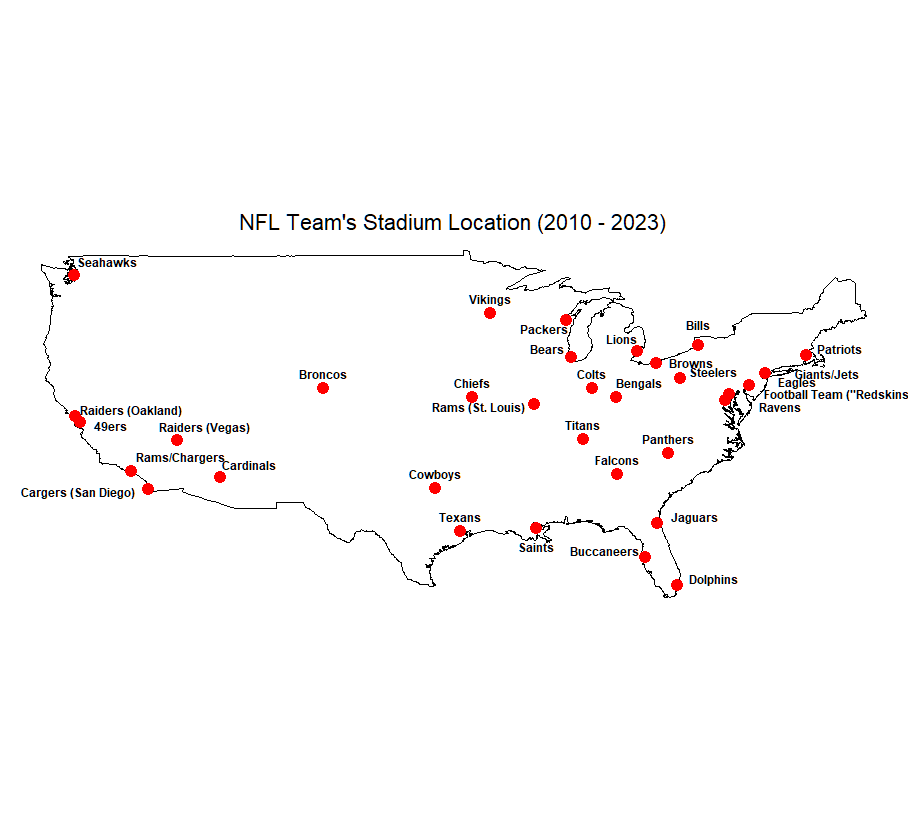
\includegraphics[scale=0.75]{Location.jpg}
\end{figure}
\section{Further Tables}


\end{document}
